%%%%% START PREAMBLE HEADER %%%%%

%%% START REQUIRED PACKAGES %%%

\documentclass[twocolumn]{article}
\usepackage[a4paper, total={7.25in, 9.5in}]{geometry} 
\usepackage{multirow}
\usepackage{multicol}
\usepackage{lipsum}
\usepackage{hyperref}
\usepackage{listings}
\usepackage{graphicx}
\usepackage{import}
\usepackage[table,xcdraw]{xcolor}
\usepackage[export]{adjustbox}
%\usepackage[superscript,biblabel]{cite}
\usepackage{amsmath}
\hypersetup{colorlinks=true,linkcolor=blue,filecolor=magenta,urlcolor=cyan,citecolor=blue}

%%% END REQUIRED PACKAGES %%%                


%%% START NEW COMMANDS new (shortcut) %%%

% This is a paragraph with normal font
\newcommand{\np}[1]{\paragraph*{\normalfont{#1}}}
% This is a text with a color
\newcommand{\ct}[2]{\textcolor{#1}{#2}}
% This is a bold text 
\newcommand{\bt}[1]{\textbf{#1}}
% This is an italic text 
\newcommand{\et}[1]{\emph{#1}}
% This is an underline text 
\newcommand{\ut}[1]{\underline{#1}}
% This is a newline shortcut
\newcommand{\n}{\\}
% This is a numbered equation with break line shortcut
\newcommand{\necbreak}[1]{\begin{equation}\begin{aligned}#1\end{aligned}\end{equation}}
% This is a numbered equation with break line shortcut
\newcommand{\nec}[1]{\begin{equation}#1\end{equation}}
% This is an equation shortcut
\newcommand{\ec}[1]{\begin{center} $#1$ \end{center}}
% Table title with bold text and correct space%
\newcommand{\titleTable}[2]{\np{\bt{Table #1} #2}}% Graph title with bold text and correct space%
\newcommand{\titleGraph}[2]{\np{\bt{Graph #1} #2}}
% Table body with border %
\newcommand{\bodyTable}[2]{\begin{center} \begin{tabular}{|#1|} \hline #2 \hline \end{tabular} \end{center} }
%%% END NEW COMMANDS (shortcuts) %%%


%%% START TITLE SETTINGS %%%
\title{\bt{Practice \# 3 Thermodynamic corrections and the contribution of entropy, addition reaction of ethene with hydroxyl radical.}}
\author{Pérez Alvarado Luis Raymundo, School of Chemistry, UNAM}
\date{21/01/2021}
%%% END TITLE SETTINGS %%%

%%%%% END PREAMBLE HEADER %%%%%

%%%%%%%%%%%%%%%% START DOCUMENT %%%%%%%%%%%%%%%%
\begin{document}

    %%% THIS CONTENT IS IN ONE COLUMN (START) %%%
    \twocolumn[
        \begin{@twocolumnfalse}

            %% CREATE A TITLE (START) %%
            \maketitle
            %% CREATE A TITLE (END) %%

            %% CREATE A ABSTRACT (START,MAX 250 CHARACTERS) %%
            \begin{abstract}
                \item The addition reaction of ethene with hydroxyl radical was analyzed and compared with the reaction of elimination of methane with hydroxyl radical, using the methods HF, B3LYP, M052X, and M062X we can corroborate that HF does not work for kinetics studies were corroborate the importance of the thermodynamics corrections in calculations of computational chemistry, also the relevance of considering the entropy contribution in the reaction, the reason why can not use the approximation of $\Delta G \approx \Delta H$ in bimolecular reactions.
                \item \bt{Keywords:}\em{ reaction profile, thermodynamic corrections, bimolecular reacction..}
            \end{abstract}
            %% CREATE A ABSTRACT (END) %%
    
        \end{@twocolumnfalse}
    ]
    %%% THIS CONTENT IS IN ONE COLUMN (END) %%%

    %%% THIS CONTENT IS IN TWO COLUMN (START) %%%

    %% START SECTION %%

    % SECTION TITLE %
    \section*{Introduction $\small{^{\cite{web:thermo}}}$ }
    
    \np{Gaussian program is capable of computing thermodynamics properties of a molecular system to model chemical reactions, these are calculated using partition function for ideal gas obtained from the statistical thermodynamic.}

    \np{After computing the electronic energy $\epsilon_0$ of the system, is necessary to add a thermodynamics correction to this result, giving as a thermodynamic property the sum of electronic energy and correction,this sum is used as the property.}

    \np{These are the properties with his corrections given by gaussian.}

    \np{sum of electronic and zero point energies = $\epsilon_0+\epsilon_{ZPE}$\\
        sum of electronic and thermal energies = $\epsilon_0+E_{tot}$\\
        sum of electronic and thermal enthalpies = $\epsilon_0+H_{corr}$\\
        sum of electronic and thermal free energies = $\epsilon_0+G_{corr}$
    }

    \np{Breaking down these fixes}

    \nec{H_{corr}=E_{tot}+K_bT \label{eq:1}}
    \nec{G_{corr}=H_{corr}-TS_{tot} \label{eq:2}}   

    \np{Where the $E_{tot}$ is the total energy of the system and $k_b$ Boltzman constant.}

    \np{An approximation can be done $\Delta ZPE \approx \Delta H \approx \epsilon_0$ in general because his values are very nearly.}

    \np{Also can be equal to $\Delta G$ in unimolecular reaction, in this case the mean error is about 1.5 kcal/mol of the experimental value which is acceptable for a calculation.}

    \np{But in bimolecular reactions, the entropy decreases by the formation of the reaction complex, and when a single product is formed, for this reason, can not use the approximation $\Delta H \approx \Delta G$.}

    \np{This study, is calculated the oxidation of ethene with hydroxyl radical \cite{art:reaction} to check the importance of thermodynamics corrections and corroborate if approximations are near to experiential values.}

    \nec{
        C_2H_2 + \cdot OH \rightarrow \cdot C_2H_2OH \label{eq:3}
    }

    \section*{Materials and methods}

    \np{The modeling of the systems $C_2H_2$, $\cdot OH$, transition state $(TS)$ and $\cdot C_2H_2OH$ was performed with gaussView separately.}

    \np{The calculations were performed with a laptop with an i7-8750H processor with 8GB of RAM.}

    \np{The transition state is describe in \eqref{eq:4} and represent in figure 1.\n}

    % START FIGURE %
    \begin{figure}[h!]
        % Reactive %
        \centering
        \begin{minipage}[b]{0.225\textwidth}
            \centering
          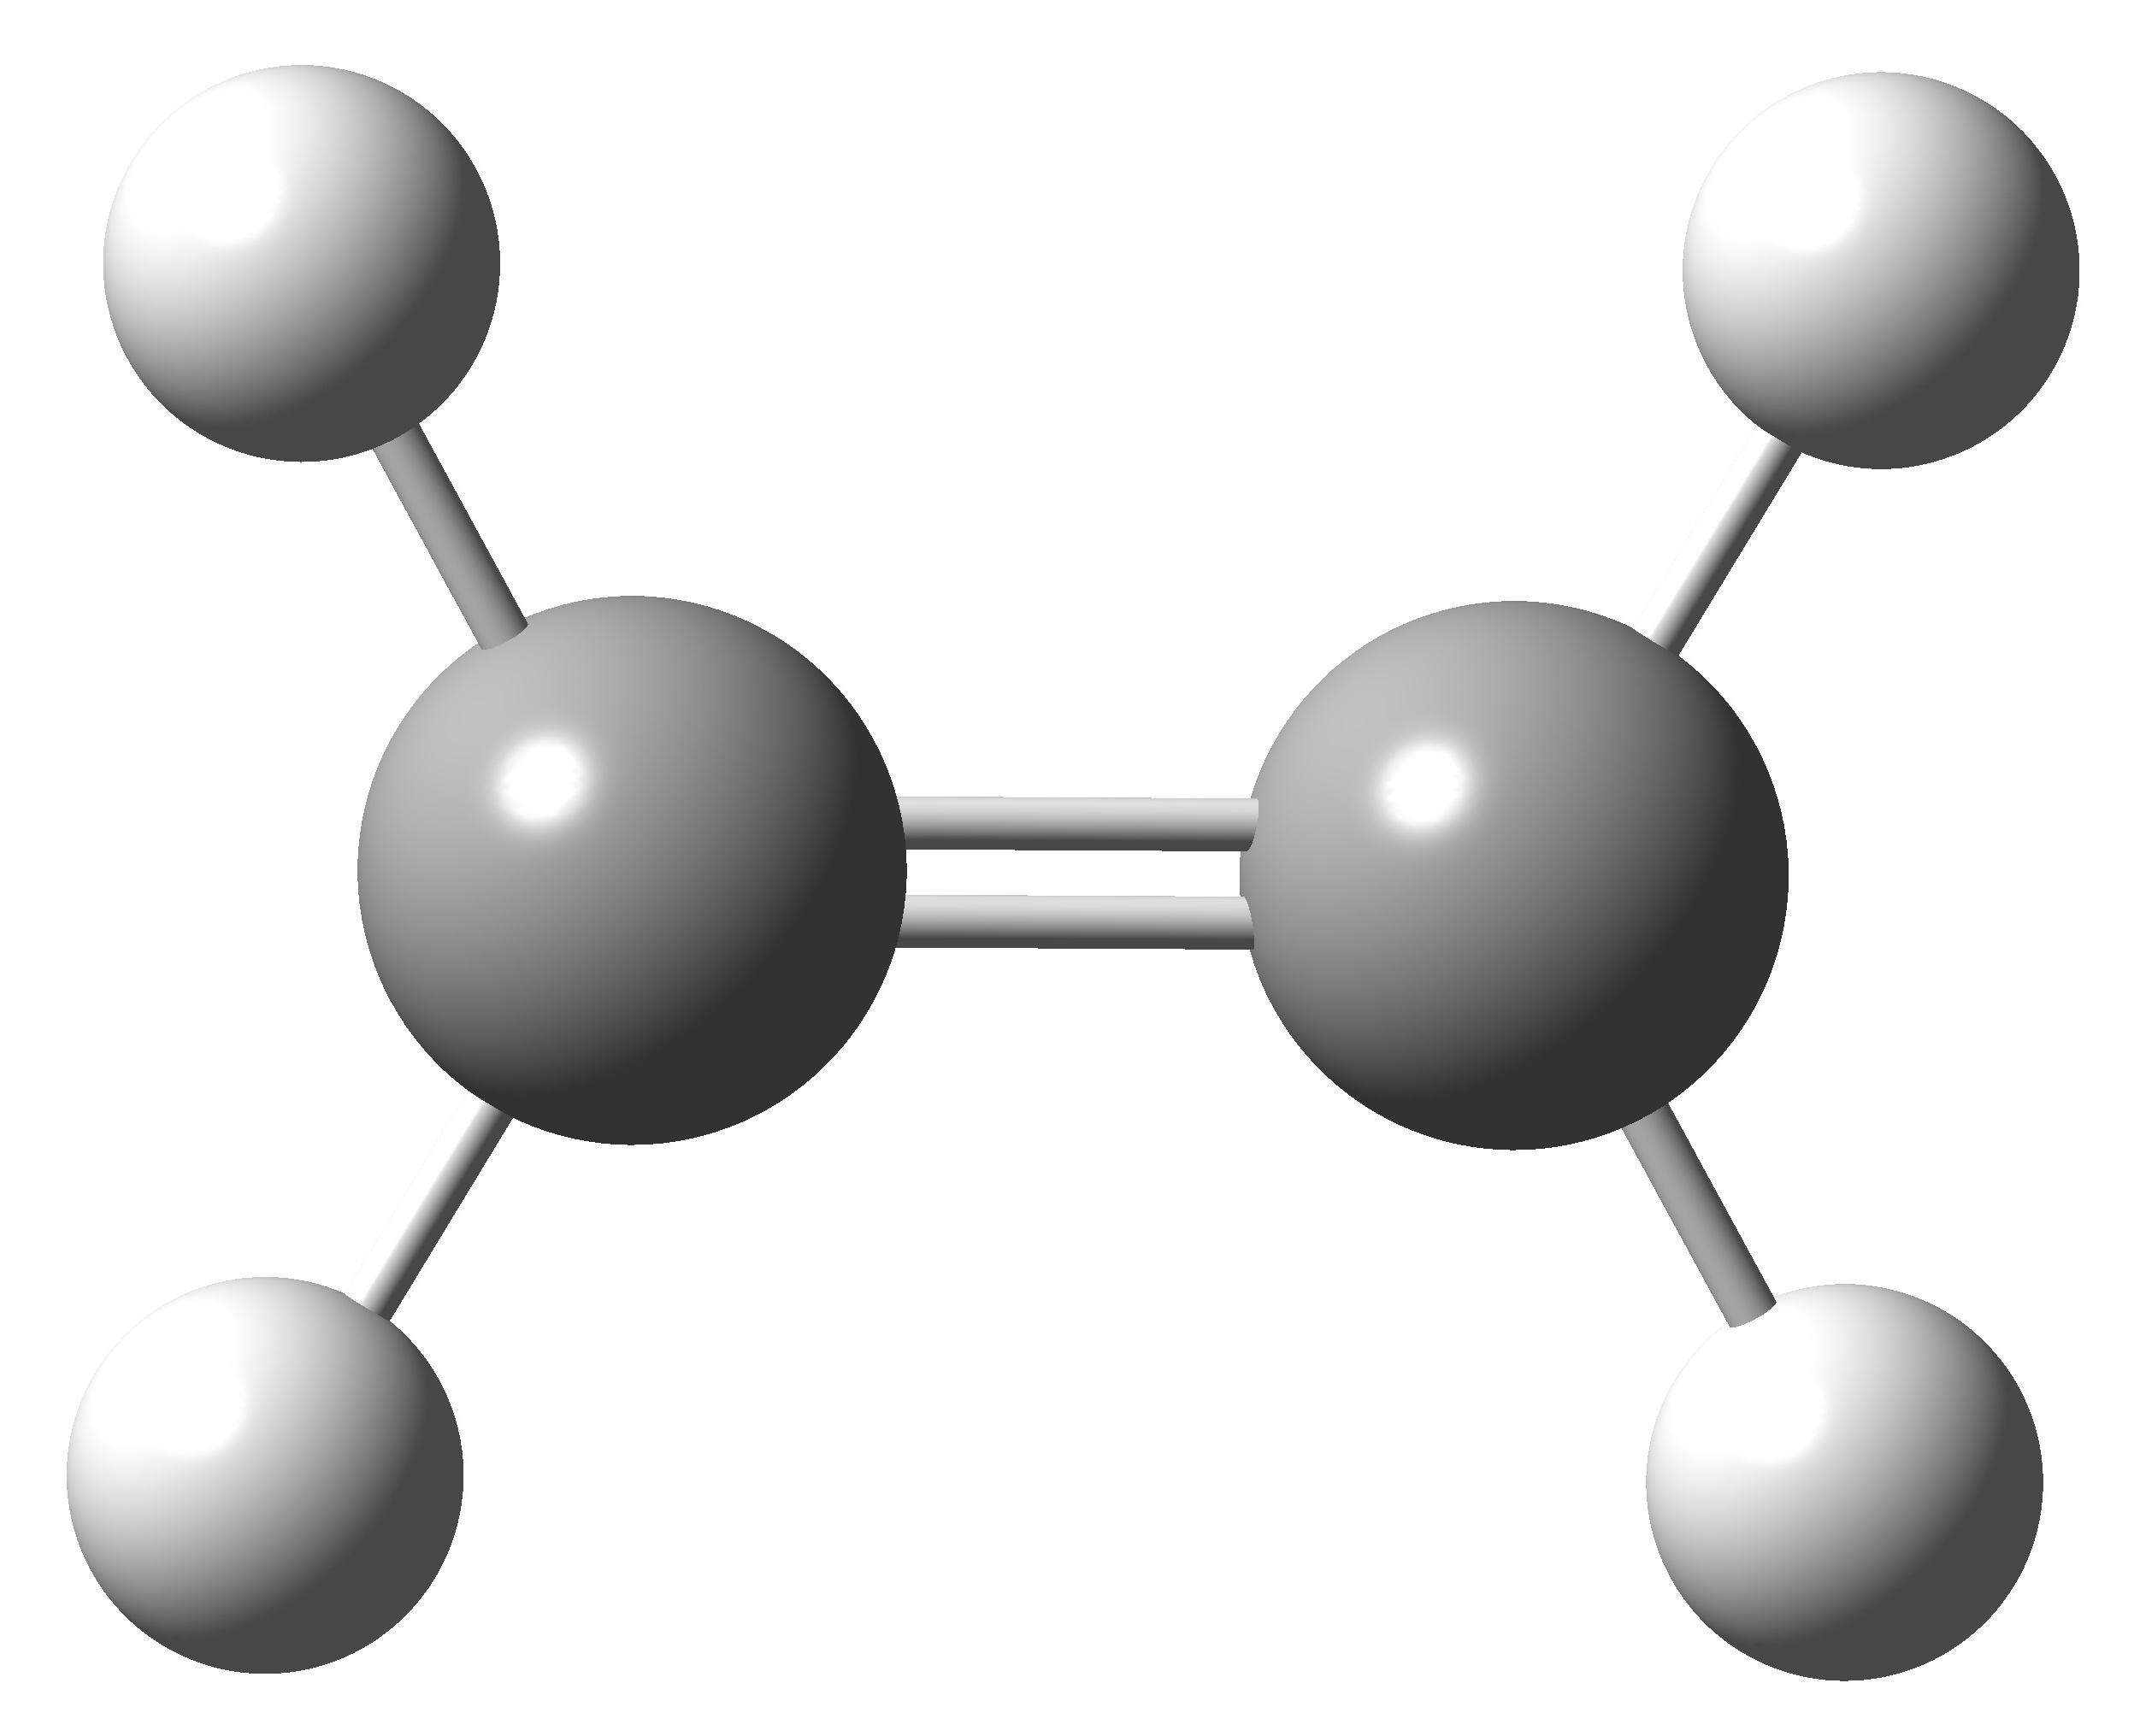
\includegraphics[scale=0.07]{ethene.jpg}
          \caption{Ethane.}
        \end{minipage}
        \hfill
        \begin{minipage}[b]{0.225\textwidth}
          \centering
          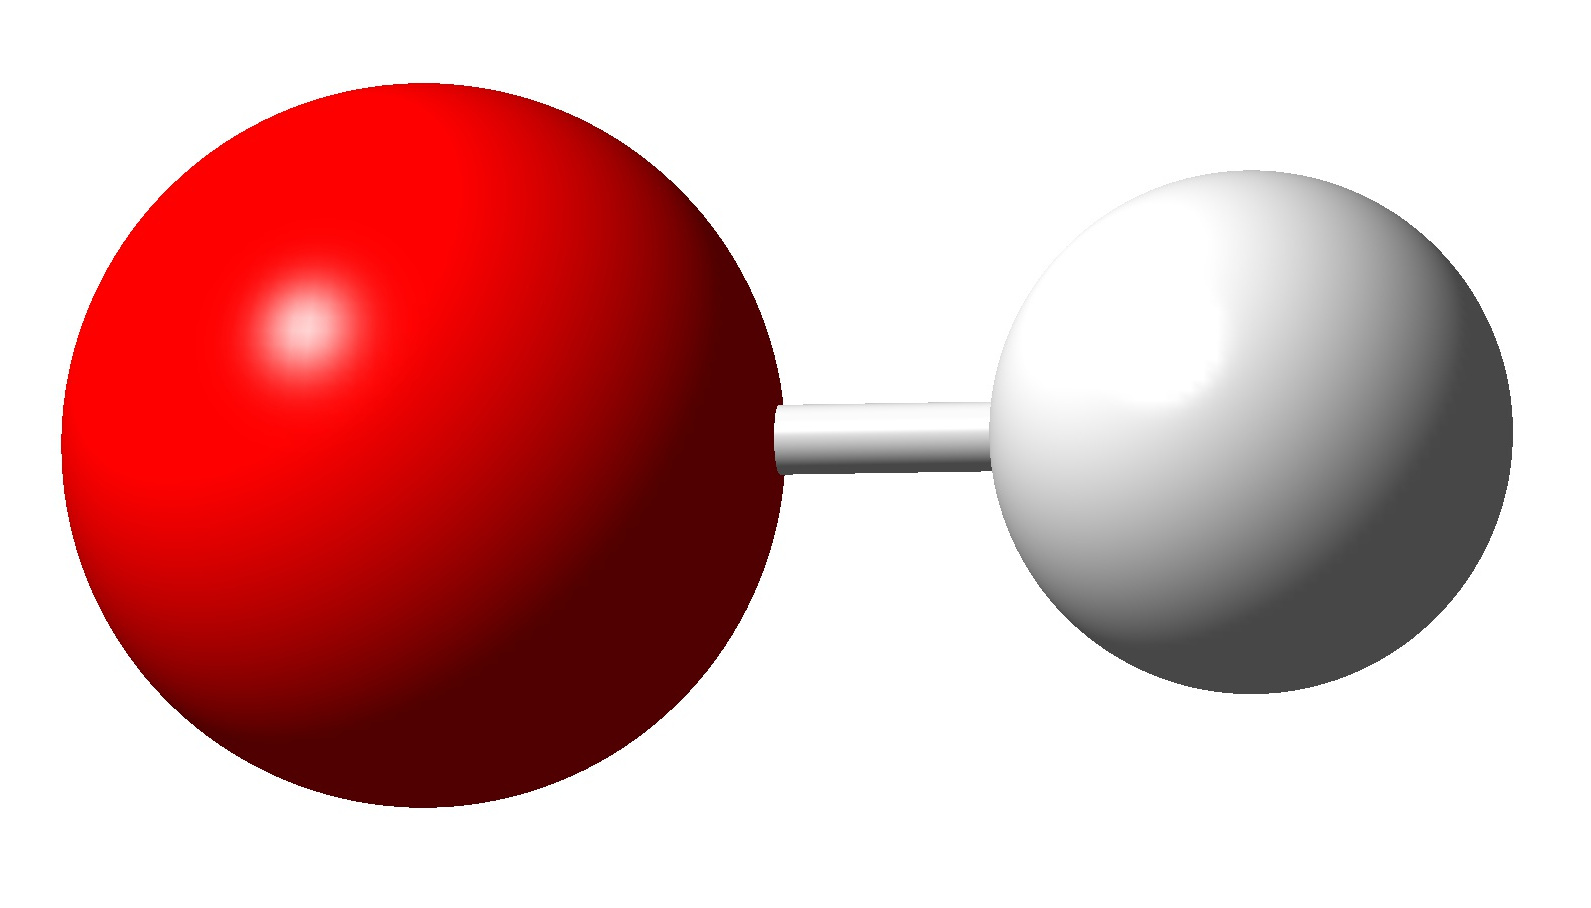
\includegraphics[scale=0.08]{hydroxyl.jpg}
          \caption{Hydroxyl radical.}
        \end{minipage}
        %Transition state%
        \begin{minipage}[b]{0.45\textwidth}
            \centering
            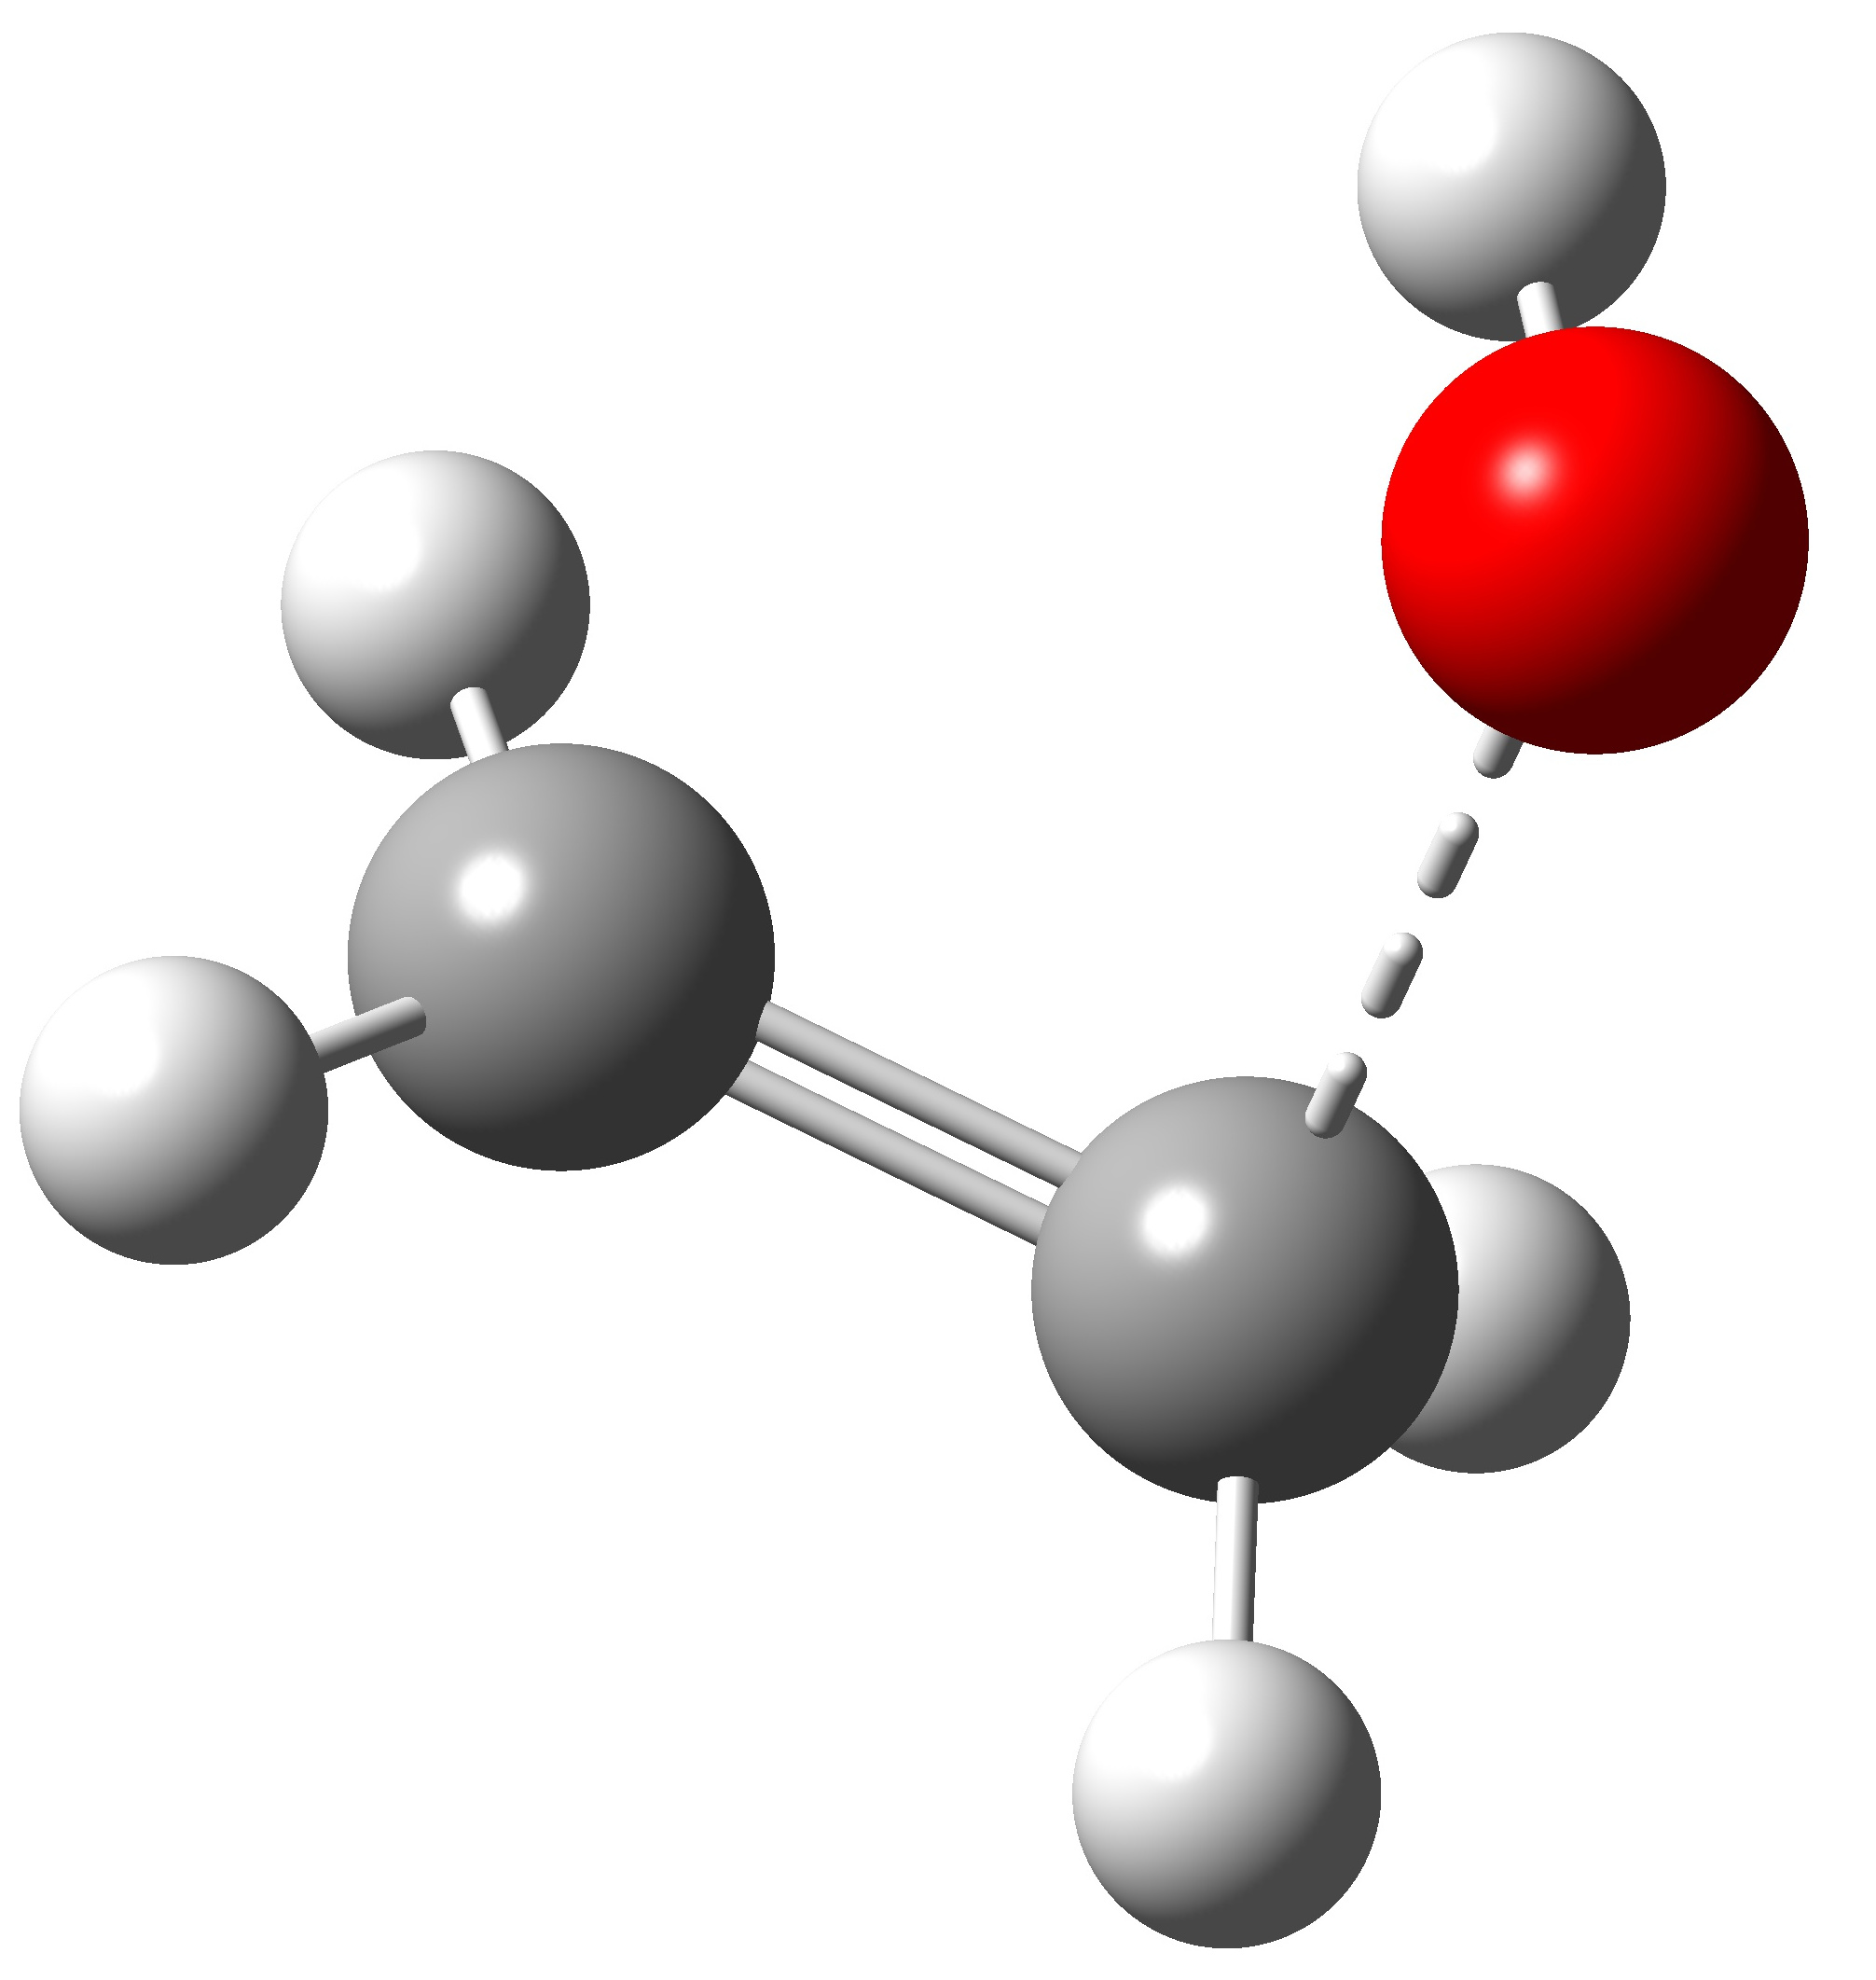
\includegraphics[scale=0.125]{ts.jpg}
            \caption{Transition state.}
        \end{minipage}
        \hfill
        \begin{minipage}[b]{0.45\textwidth}
          \centering
          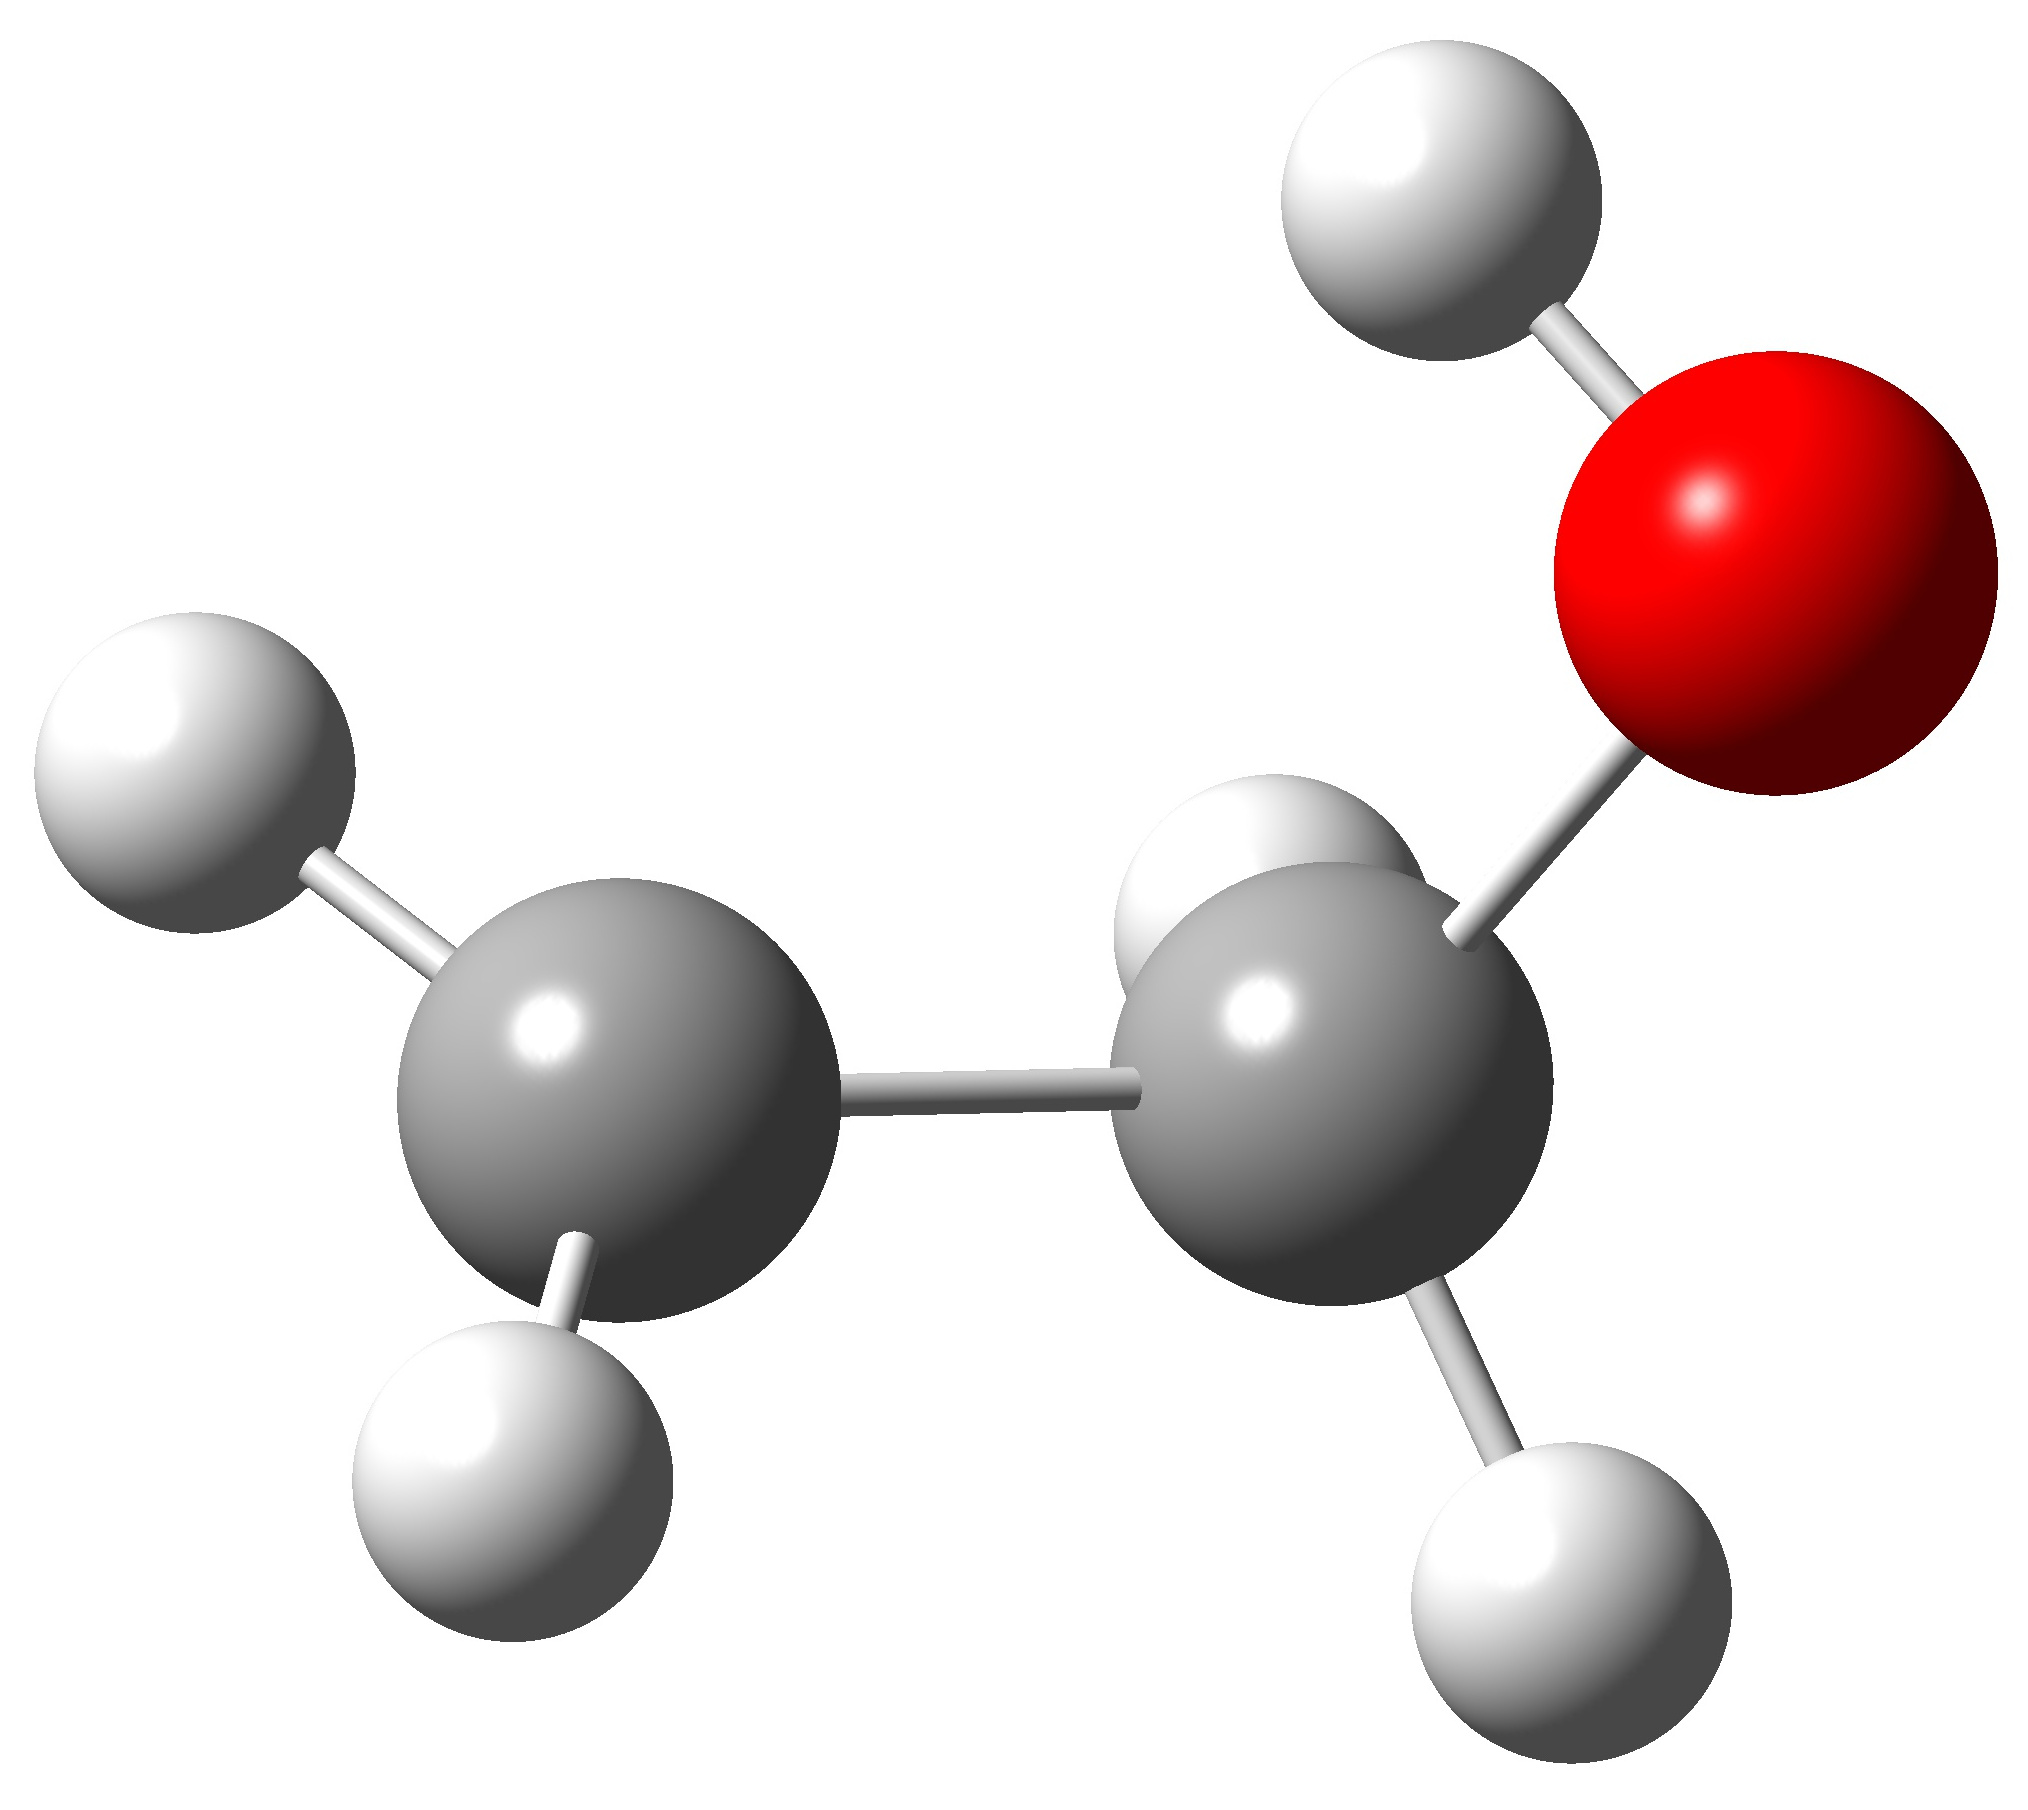
\includegraphics[scale=0.125]{prod.jpg}
          \caption{2-Hydroxyethyl.}
        \end{minipage}
    \end{figure}
    % END FIGURE %

    \nec{ C_2H_2 + \cdot OH \rightarrow [H_2CH_2C\mbox{-}\mbox{-}\mbox{-}OH]^{\ddag} \label{eq:4}
    }

    \np{The input file of reactives and products was running with the following settings. \n \n \n}

    \begin{lstlisting}[frame=single,gobble=10] 
            //hardware configuration
            % nprocshared=4
            % mem=1500MB
            //parameters for Method and bases set
            # opt freq 6-31+G(d,p) X
    \end{lstlisting}

    \np{X = [HF, B3LYP, M052X and M062X] are the methods used and they were run with the bases set 6−31+G(d,p).}
    
    \np{For transition state was calculated with the following settings.\n}

    \begin{lstlisting}[frame=single,gobble=10] 
            //parameters for method
            # opt=(calcfc,ts,noeigen)
            freq=noraman 6-31+g(d,p) 
            iop(1/8=3) X
    \end{lstlisting}    
    
    \np{\bt{NOTE:} In the calculation of transition state was necessary to run twice the system because the system did not converge, in these cases, we re-run the last configuration and run the following command \em{\# opt=(readfc,ts,noeigen) geom=check guess=check freq=noraman 6-31+g(d,p) iop(1/8=3) X}.}
    
    \section*{Results}
    
    \np{The computed results are shown in table 1 in the appendix, in table 2 we show the processed data to build the reaction profile and table 3 shows the data used for the profile reaction.}

    \titleTable{3}{Reaction profile with $\Delta G$, $\Delta H$, $\Delta ZPE$ in $\frac{kcal}{mol}$.}

    \begin{center} 
        \item \import{./}{table3.tex}
    \end{center}

    \np{With table 3 we build the reaction profile, using each potential.}

    \titleGraph{1}{ZPE VS Reaction coordenate \\ \\}

    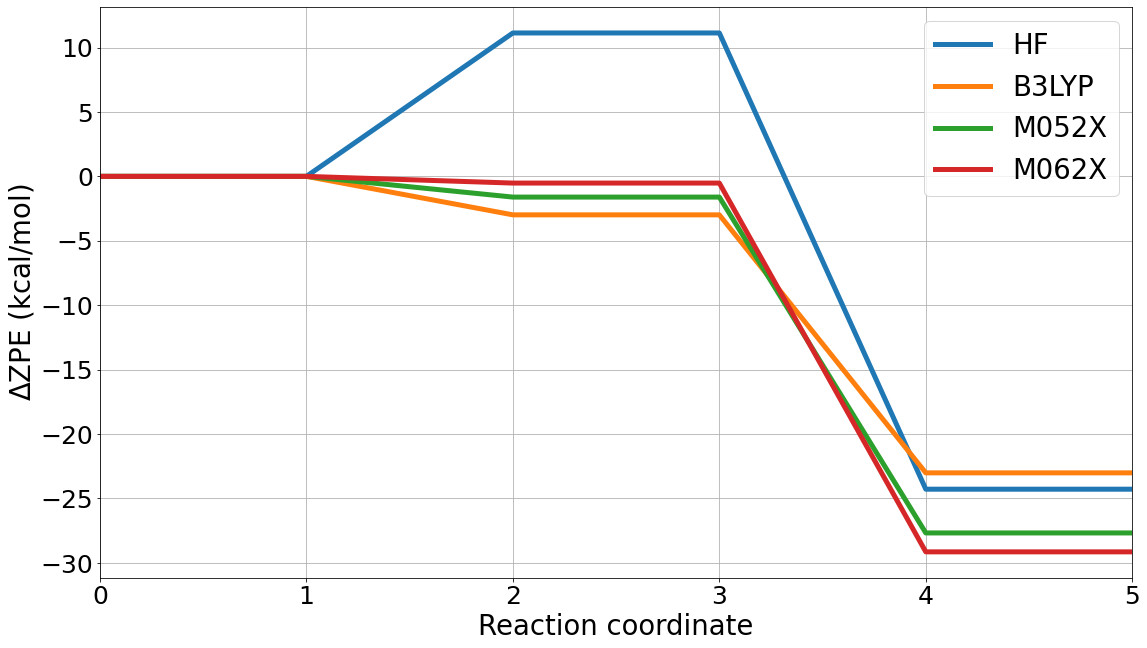
\includegraphics[width=0.5\textwidth]{zpe}

    \titleGraph{2}{Enthalpy VS Reaction coordenate \\ \\}

    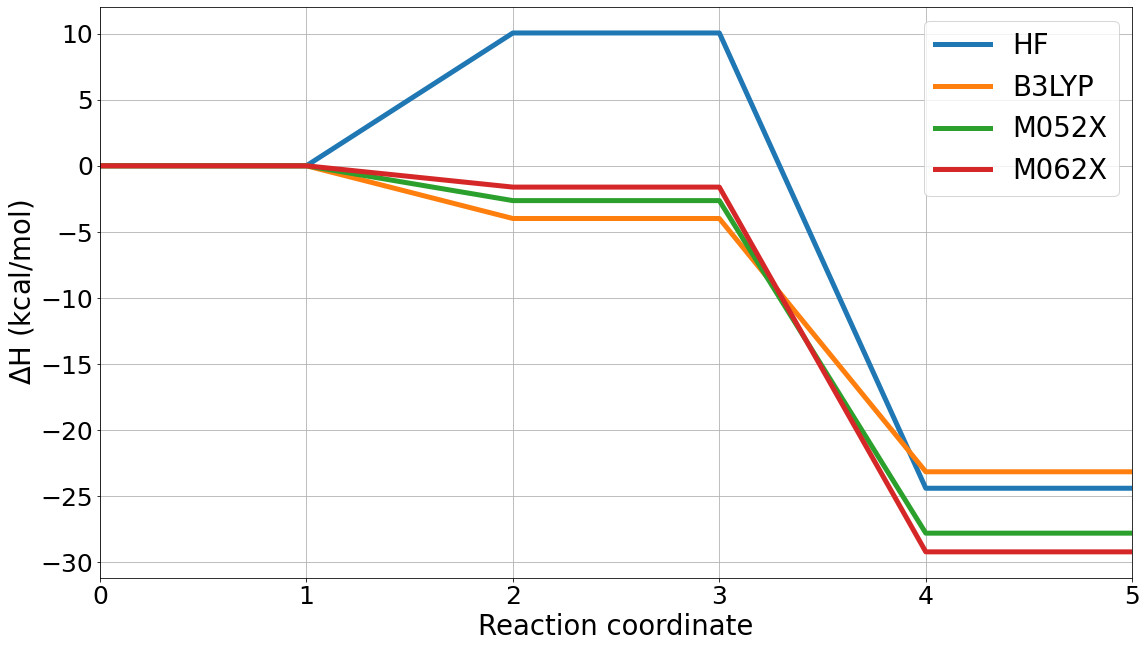
\includegraphics[width=0.5\textwidth]{h}

    \titleGraph{3}{Free energy VS Reaction coordenate \\ \\}

    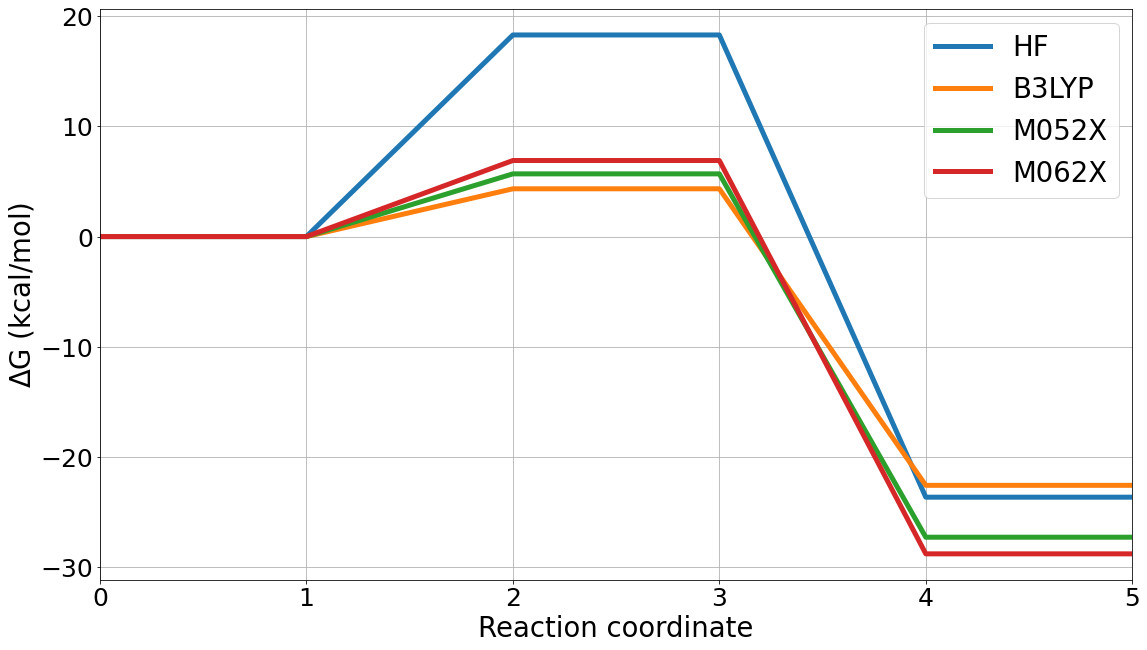
\includegraphics[width=0.5\textwidth]{g}


    \np{In the following graph were plot the values of $\Delta G$ and $\Delta H$ of the current reaction and the reaction of hydroxyl radical with methane.}

    \titleGraph{4}{Free energy and Enthalpy VS Reaction coordenate \\ \\}

    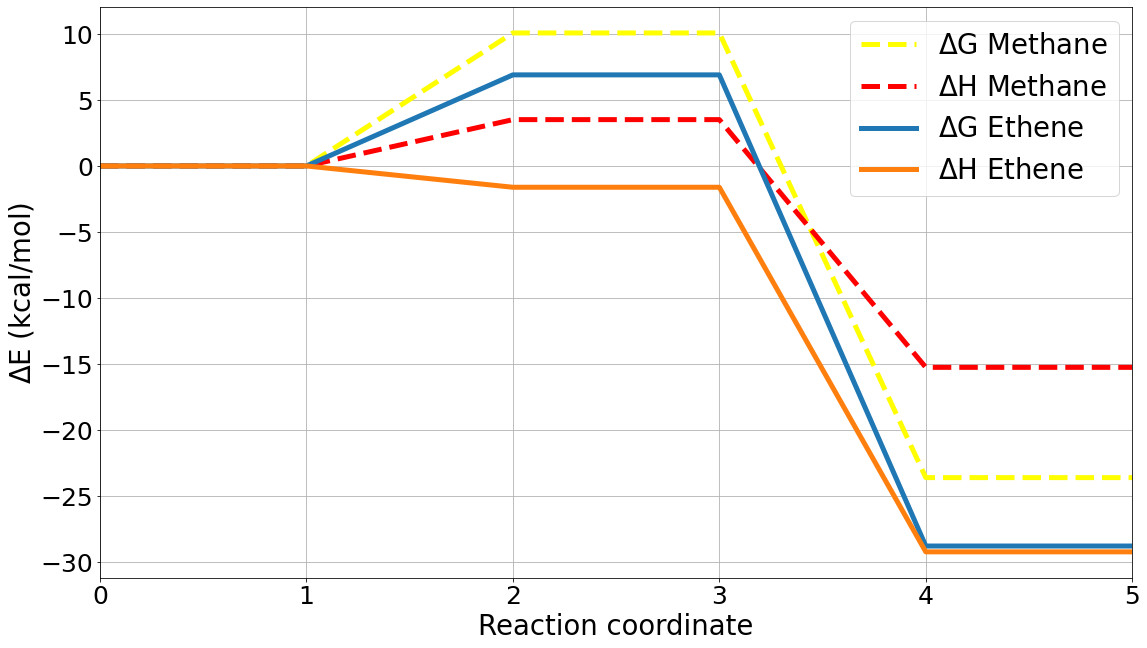
\includegraphics[width=0.5\textwidth]{comparation.jpg}

    \np{Rate constant was calculated with Eyring equation \cite{web:Eyring_equation} for each method, was considered $\kappa=1$ and $\sigma=4$ at 1 atm of pressure, with the experimental value of the rate constant we compared the results $5.02E+09 (s^{-1}M^-1)$ \cite{web:rate}, and sum the total time of calculation.}

    \titleTable{3}{Rate constant with HF, B3LYP and MP2.}

    \begin{center} 
         \item \import{./}{table4.tex}
    \end{center}

    \section*{Discussion}

    \np{Seeing graph 1 and 2 two facts which are that the values of $\Delta ZPE$ and $\Delta H$ are similar, and comparing the methods can be appreciated how HF overestimated the values, for this reason, can not be used for kinetics.}

    \np{Comparing graphs 2 and 3 \bt{we can corroborate the importance of thermodynamics corrections and why is not correct the approximation of $\Delta G \neq \Delta H$ for bimolecular reactions}, where the values are significantly different.}

    \np{With graph 4 we compare two bimolecular reactions where the reactant reacts with hydroxyl radical and they form a transition state but have a significant difference between them because in methane reaction are two reactive and two products, but in the reaction of ethene are just one product, in this one the number of moles decreases, this is the reason why the corrections can not be considered as equal, the consequence of this is a loss of degrees of freedom in the system this is directly a loss of entropy, and seeing \bt{$G_{corr}$ equation \eqref{eq:2} we can see that depend directly on the $\Delta S$,  so is important consider always the contribution of entropy using the $\Delta G$ and not only the $\Delta H$.}}

    \np{The rate constant was calculated for each method and is show that M052X and M062X are methods good for kinetics studies and proof how good are the calculated properties, also were compare the two methods and we can see that \bt{M062X give an excellent approximation to the experimental value}, M052X  also gives a very good value but comparing with M062X is more expensive in time and a little farther than M062X, finally, \bt{we can corroborate that a gas phase approximation can be used to calculate properties of the reaction in the gas phase with good results.}}

    %% END SECTION %%
    

    %% START REFERENCES %% 




    % DEFINE STYLE FORMAT%
    \bibliographystyle{ieeetr}
    % SPECIFY THE FILE NAMEw %
    \bibliography{references}

    %START APPENDIX (always in last page)%
    \appendix
    % CHANGE FROM X COLUMN TO ANOTHER COLUMNS EJ 2 -> 1%
    \onecolumn
    \section{Appendix}
    \begin{center}
        \item \titleTable{1}{Values of $\Delta G$, $\Delta H$, $\Delta ZPE$ and Time of running}
        \item \import{./}{anexo1.tex}
        \item \np{\em{Note:} H are Hartree units.}
    \end{center}

    \begin{center}
        \item \titleTable{2}{Values for profile of reaction of $\Delta G$, $\Delta H$, $\Delta ZPE$}
        \item \import{./}{anexo2.tex}
    \end{center}




    %% END REFERENCES %% 

    %%% THIS CONTENT IS IN TWO COLUMN (END) %%%

\end{document}
%%%%%%%%%%%%%%%% END DOCUMENT %%%%%%%%%%%%%%%%